%%%%%%%%%%%%%%%%%%%%%%%%%%%%%%%%%%%%%%%%%%%%%%%%%%%%%%%%%%%%%%%%%%%%%%%%%%%%%%%%
% experiment.tex: Chapter describing the experiment
%%%%%%%%%%%%%%%%%%%%%%%%%%%%%%%%%%%%%%%%%%%%%%%%%%%%%%%%%%%%%%%%%%%%%%%%%%%%%%%%
\chapter{Heavy Photon Search}
\label{chapter:hps:experiment}
\todo[citation]{How do I cite this HPS detector chapter? I'm mainly taking this information
	from theses but those theses cite a proposal document hosted on confluence.}

%%%%%%%%%%%%%%%%%%%%%%%%%%%%%%%%%%%%%%%%%%%%%%%%%%%%%%%%%%%%%%%%%%%%%%%%%%%%%%%%
\ac{hps} is currently installed behind the CLAS-12 experiment in the Hall B
alcove at \ac{jlab} and utilizes the \ac{cebaf} to provide its beam
\cite{mrsolt-thesis-2020,skmccarty-thesis-2020}.
Hall B primarily hosts the CLAS-12 experiment \todo[citation]{Add citation for CLAS-12}
in the bulk of its hall; nevertheless, behind the CLAS-12 experiment \ac{hps} is situated
within an alcove such that it can collect data whenever CLAS-12 is not operational (for example,
when its components are being upgraded or fixed).

\ac{cebaf} \cite{cebaf-12GeV-2012,cebaf-opportunities-2012,cebaf-2013} is able to
provide a near-continuous electron beam ranging in energy up to $12$ GeV in steps
of $\approx 1.15$ GeV. \ac{cebaf} is built in a oval ``race track'' where the straight
portions consist of linear accelerators and the curve portions steer the beam with
dipole magnets either back into the straight portions or into experimental halls.
Since \ac{cebaf} delivers electrons at such a high rate, \ac{hps} must be able to
handle these high radiation loads. Designed to be a small experiment to fit within
the Hall B alcove, \ac{hps} elected to be built in two halves that straddle the primary
path of the beam where the highest amount of radiation would be. Both of the subsystems
within \ac{hps} are split into these two halves as shown in \cref{fig:hps-full-render}
and \cref{fig:hps-diagram}.

\begin{figure}
	\centering
	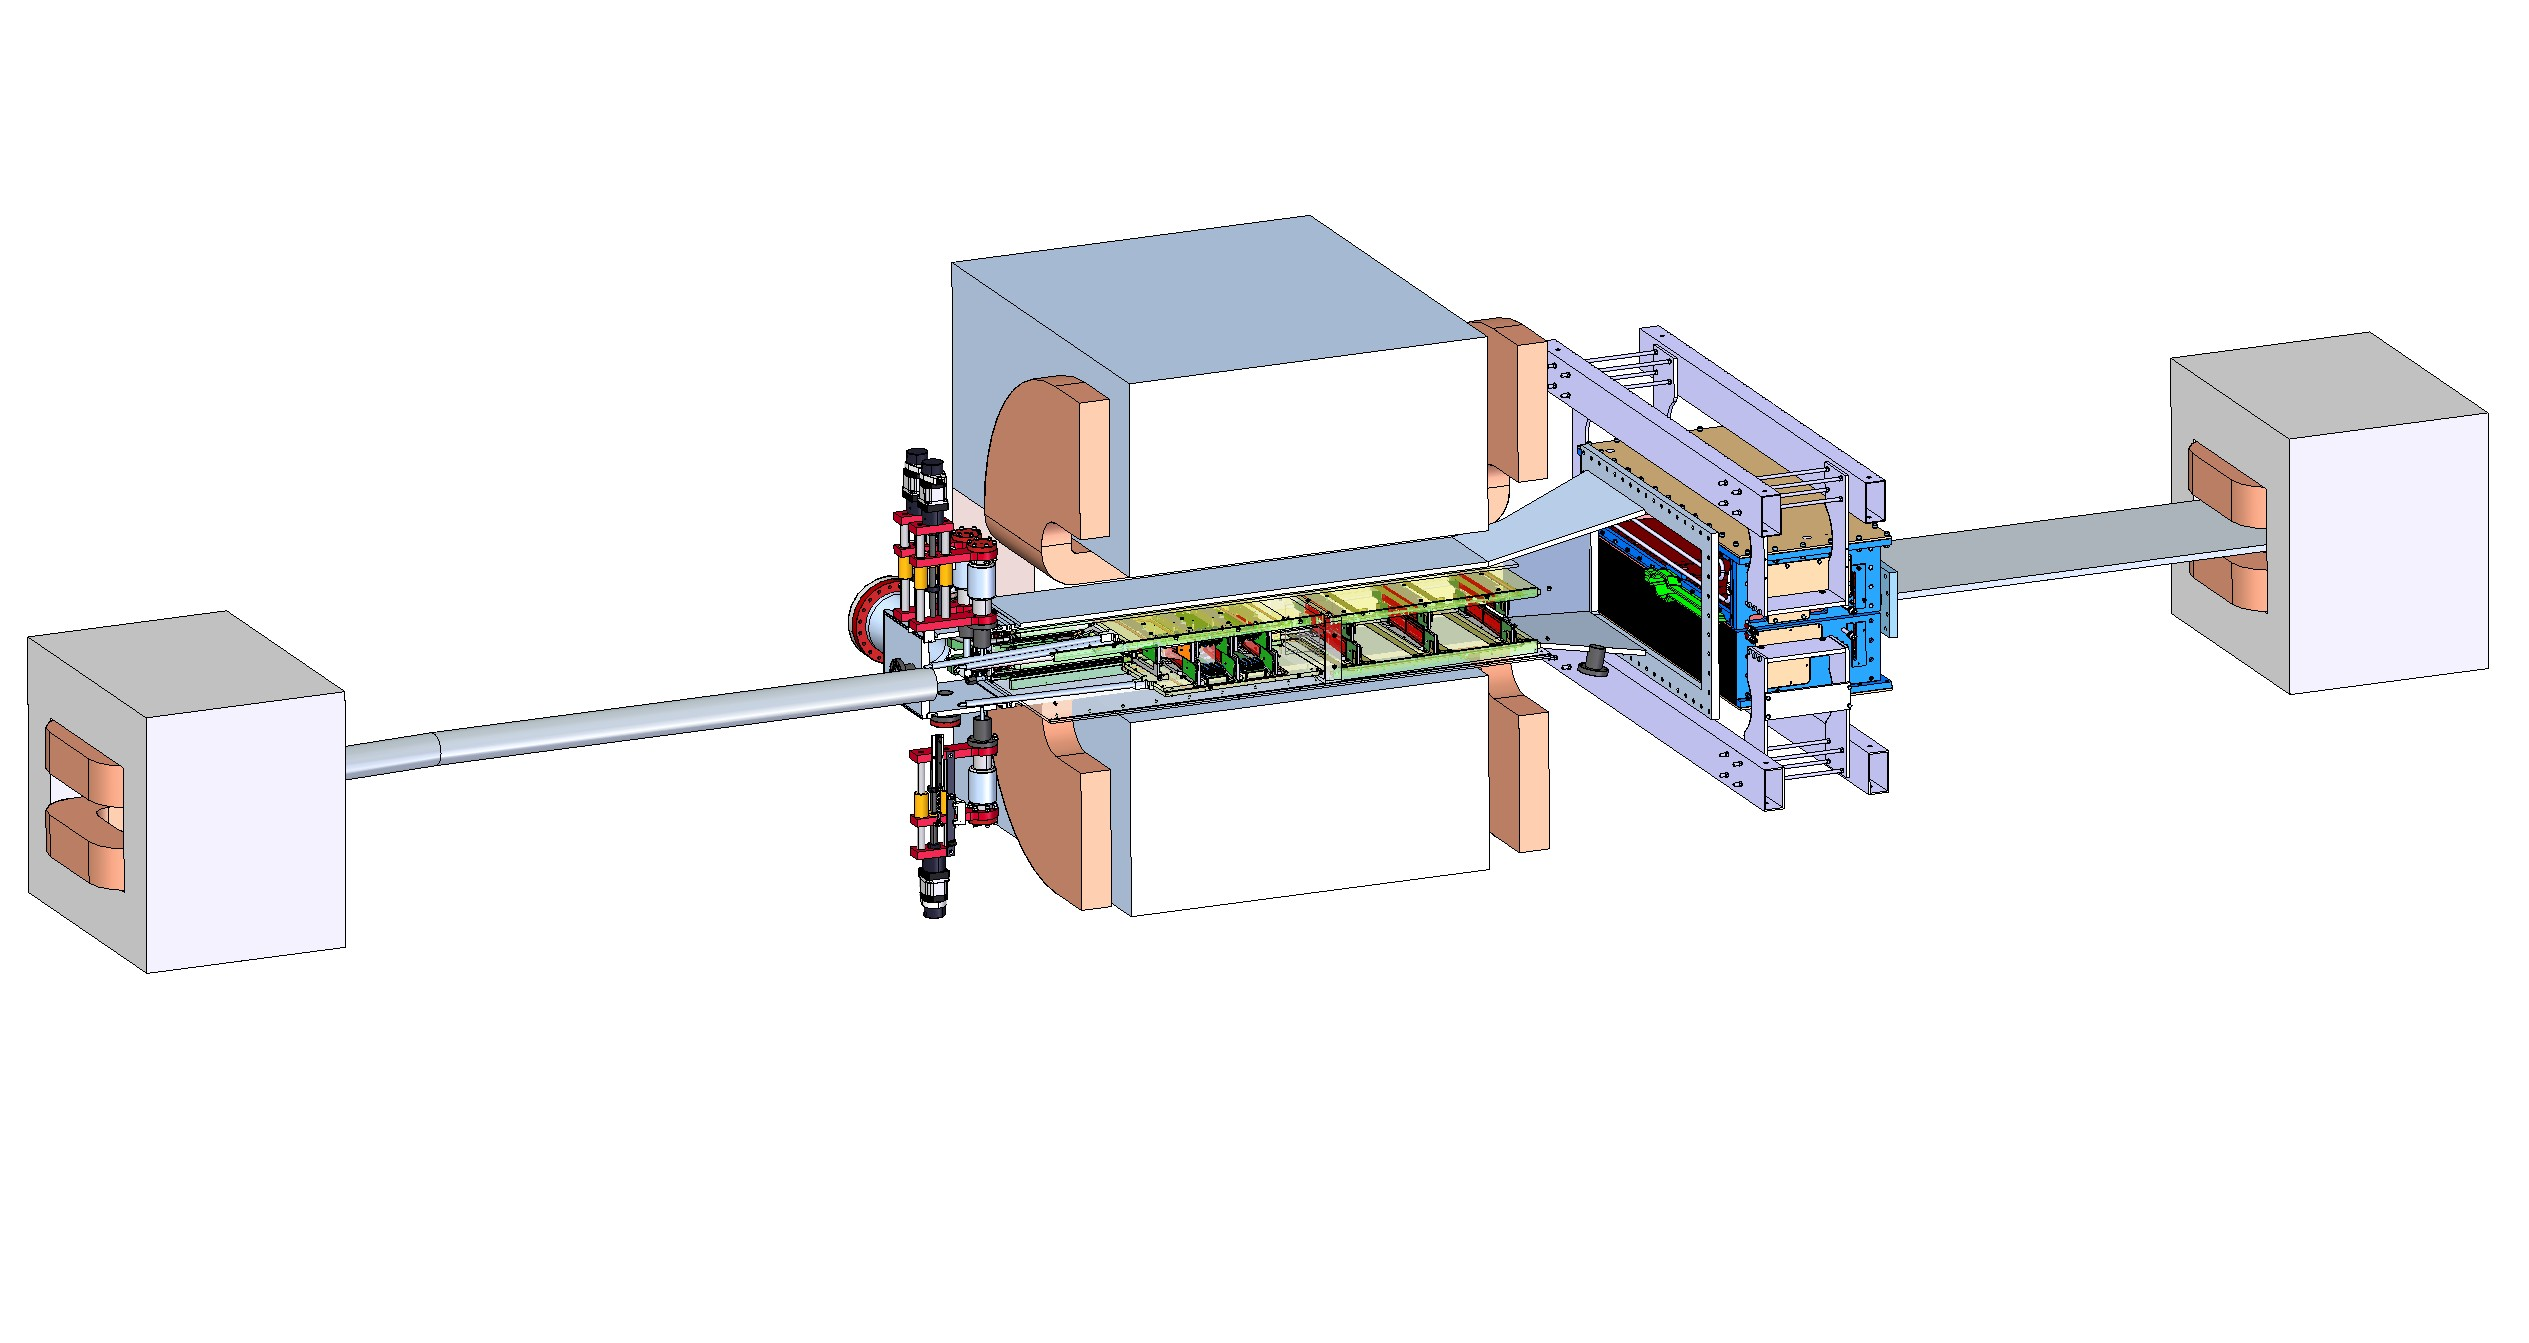
\includegraphics[trim={15cm 10cm 10cm 5cm},clip,width=\textwidth]{figures/hps/experiment/hps_full_render.jpg}
	\caption{
		Full rendering of \ac{hps}.
		Beam would enter the detector from the left and exit to the right if it does not interact.
	}
	\label{fig:hps-full-render}
\end{figure}

\begin{figure}
	\centering
	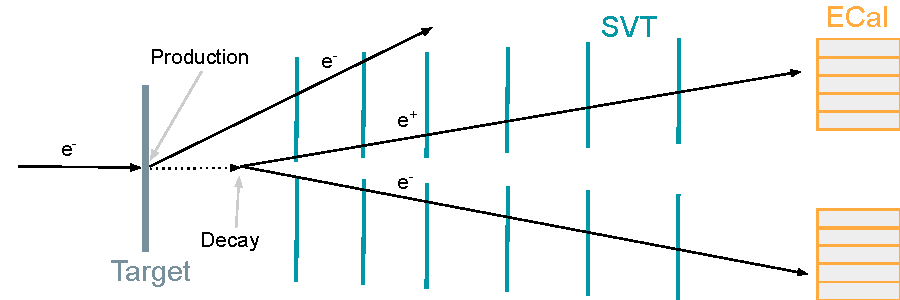
\includegraphics[width=0.9\textwidth]{figures/hps/experiment/hps-diagram.pdf}
	\caption{
		Simplified diagram of \ac{hps} showing an example displaced decay within the named subsystems.
		Not to scale.
		The dotted, unlabeled arrow is some \ac{dm} candidate particle that has a macroscopic lifetime causing
		the decay vertex to be observably displaced from the production within the target.
	}
	\label{fig:hps-diagram}
\end{figure}

\ac{hps} is designed to focus on visible signatures of \ac{dm} (\cref{sec:theory-visible}) with
a dual strategy of searching for mass resonances and displaced vertices. Both of these strategies
require precise reconstruction of a produced electron-positron pair originating from the decay of
some \ac{dm} particle. The precision of this reconstruction is one of the main limiting factors
in distinguishing whether a specific pair originated from \ac{dm} or from some other \ac{sm}
background process. The two subsystems included within \ac{hps} are the \ac{svt} focused
on reconstruction of the momentum and charge of charged particles
and the \ac{ecal} focused on energy reconstruction and online triggering of the data.

\section{Silicon Vertex Tracker}
The \ac{svt} is made of eighteen modules each of which is a pair of silicon-strip detectors
offset from each other by a small angle to enable three-dimensional position reconstruction.
The modules are arranged in the two halves separated by the center beam line. In each half,
the modules are put into layers with the first three layers consisting of one module while
the last three layers consisting of two modules to increase angular acceptance relative
to the target. \cref{fig:hps-svt-render} shows a rendering of the \ac{svt} with the sensitive
detector elements shown as red rectangles.\todo[caveat]{Should I include the detail that
	this description of the HPS SVT is for 2016 and before? An additional layer was included
	for later runs.}

The two halves of the \ac{svt} are positioned to form a \qty{15}{\milli\radian} angular gap relative
to the target in order to avoid the largest amount of radiation from the beam. The first layer
(closest to the target, left size of \cref{fig:hps-svt-render}) is placed \qty{10}{\cm} from
the target and \qty{0.5}{\mm} from the beam line in order to maximize acceptance. The entire
\ac{svt} is enclosed in a vacuum box to limit secondary production of particles and is liquid
cooled to help prevent radiation damage.

The \ac{svt} modules are readout by APV25 chips which report six samples every \qty{24}{\ns}.
These samples are only dumped to disk upon receiving a trigger signal from the calorimter
system (\cref{sec:hps-ecal}).

All together, the \ac{svt} has been observed to have \num{10}~\% momentum resolution,
\qty{2.4}{\ns} time resolution, and \qty{6}{\micro\meter} position resolution. These
properties enable the necessary momentum and vertex reconstruction for \ac{dm} searches
via visible decays.

\begin{figure}
	\centering
	\includegraphics*[width=\textwidth]{figures/hps/experiment/smkcarty-thesis-fig-10-svt-render.png}
	\caption{
		Figure 10 of \cite{skmccarty-thesis-2020}. Rendering of the \ac{svt} with the vacuum
		enclosure shown in gray, active silicon components in red, and readout electronics in
		green. Similar to \cref{fig:hps-full-render}, the beam would traverse this rendering
		from left to right.
	}
	\label{fig:hps-svt-render}
\end{figure}

\section{Electromagnetic Calorimeter}
\label{sec:hps-ecal}
The \ac{ecal} consists of \num{442} lead-tungstate crystals and is a fully-sensitive calorimeter.
The crystals are arranged in symmetric grids separated by the beamline similar to the \ac{svt}.
\cref{fig:hps-pair-trigger-depiction} shows this grid in addition to example clusters and \ac{ecal}-related
variables. In addition to a horizontal gap separating the halves, a few more crystals in the highest
radiation area are removed to form a ``hole'' to allow the majority of non-interacting (or minimally interacting)
beam electrons to pass through the detector volume. The calorimeter is sized to fit the same
angular acceptance as the \ac{svt} located \qty{139}{\cm} away from the target.

As mentioned above, one of the primary purposes of the \ac{ecal} is to be the triggering mechanism
for data collection. Many different trigger algorithms with different purposes have been used within
\ac{hps} and the specific trigger algorithm designed for collection of data relevant to a \ac{dm}
search is studied and motivated in detail in \cite{skmccarty-thesis-2020}.

\section{Currently-Available Datasets}

\begin{figure}
	\centering
	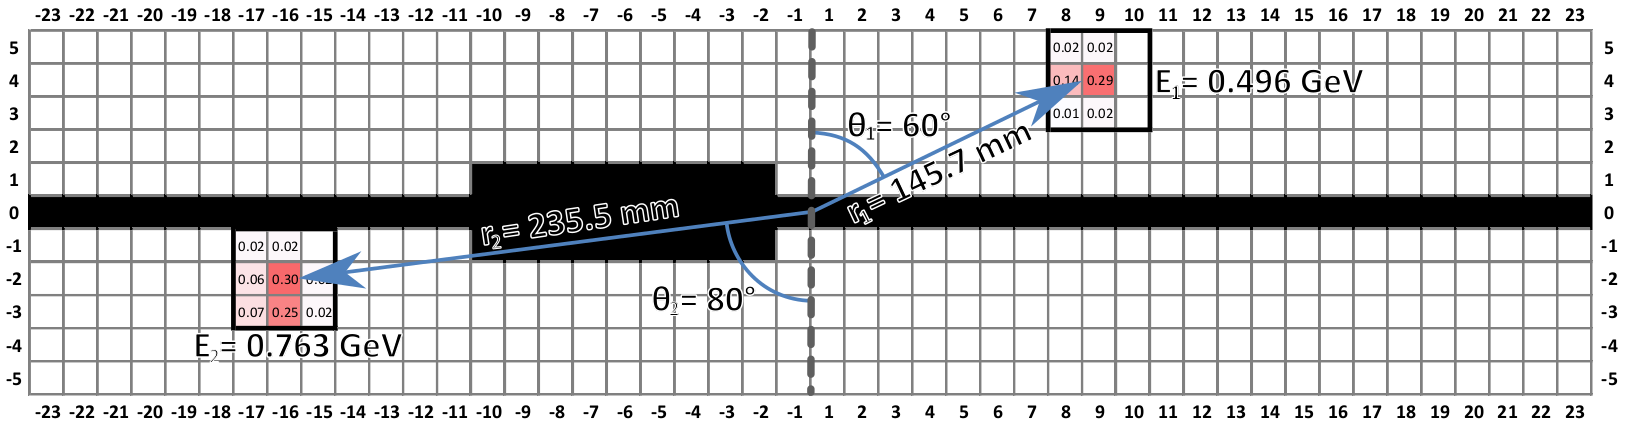
\includegraphics[width=\textwidth]{figures/hps/experiment/smckarty-thesis-fig-27-pair-trigger-depiction.png}
	\caption{
		Figure 27 of \cite{skmccarty-thesis-2020}. Depiction of an event passing the pair trigger
		in the 2016 data collection run. This depiction also displays the variables used in order
		to evaluate events and make the trigger decision.
	}
	\label{fig:hps-pair-trigger-depiction}
\end{figure}